% This file was created with matplot2tikz v0.4.2.
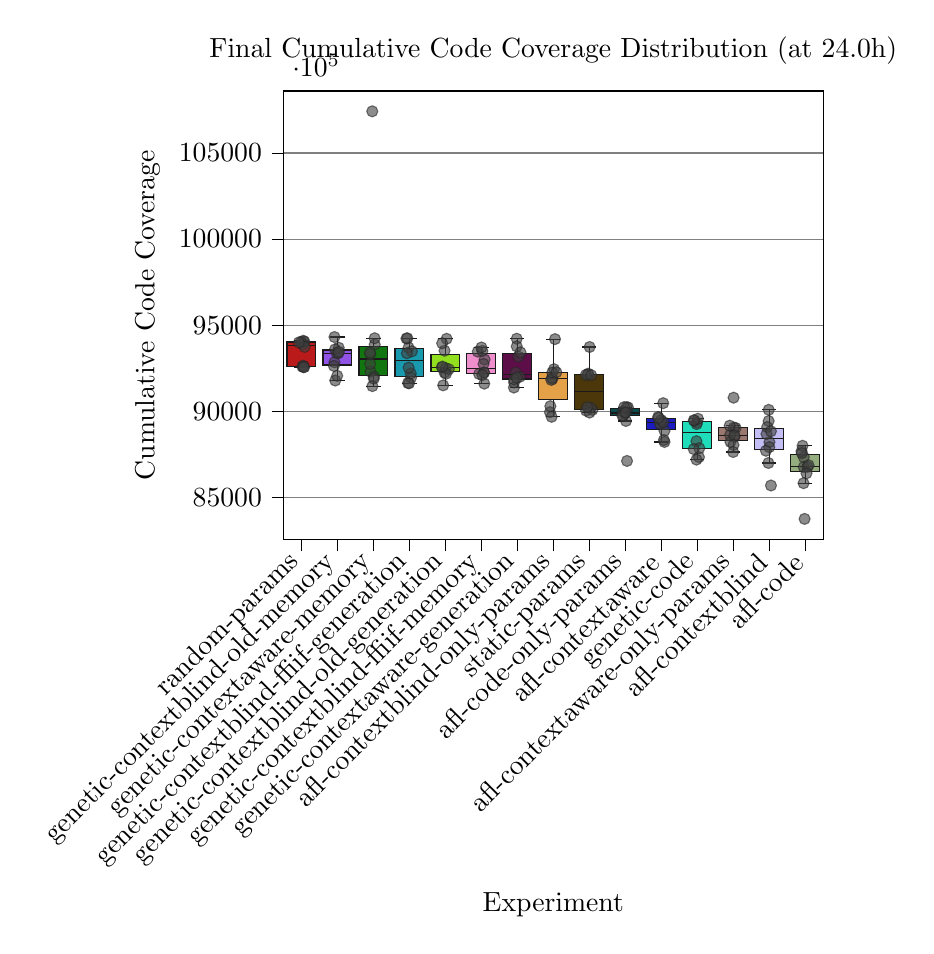
\begin{tikzpicture}

\definecolor{black26}{RGB}{26,26,26}
\definecolor{darkgray176}{RGB}{176,176,176}
\definecolor{darkolivegreen765510}{RGB}{76,55,10}
\definecolor{darkseagreen149173126}{RGB}{149,173,126}
\definecolor{darkslategray117577}{RGB}{11,75,77}
\definecolor{darkslategray38}{RGB}{38,38,38}
\definecolor{firebrick1872626}{RGB}{187,26,26}
\definecolor{gray}{RGB}{128,128,128}
\definecolor{gray154120111}{RGB}{154,120,111}
\definecolor{green1711816}{RGB}{17,118,16}
\definecolor{indigo931372}{RGB}{93,13,72}
\definecolor{lightseagreen24153173}{RGB}{24,153,173}
\definecolor{lightsteelblue195191245}{RGB}{195,191,245}
\definecolor{mediumblue2727193}{RGB}{27,27,193}
\definecolor{mediumslateblue14483230}{RGB}{144,83,230}
\definecolor{plum238142204}{RGB}{238,142,204}
\definecolor{sandybrown22916172}{RGB}{229,161,72}
\definecolor{turquoise31221186}{RGB}{31,221,186}
\definecolor{yellowgreen14522331}{RGB}{145,223,31}

\begin{axis}[
tick align=outside,
tick pos=left,
title={Final Cumulative Code Coverage Distribution (at 24.0h)},
x grid style={darkgray176},
xlabel={Experiment},
xmin=-0.5, xmax=14.5,
xtick style={color=black},
xtick={0,1,2,3,4,5,6,7,8,9,10,11,12,13,14},
xticklabel style={rotate=45.0,anchor=east},
xticklabels={
  random-params,
  genetic-contextblind-old-memory,
  genetic-contextaware-memory,
  genetic-contextblind-ffiif-generation,
  genetic-contextblind-old-generation,
  genetic-contextblind-ffiif-memory,
  genetic-contextaware-generation,
  afl-contextblind-only-params,
  static-params,
  afl-code-only-params,
  afl-contextaware,
  genetic-code,
  afl-contextaware-only-params,
  afl-contextblind,
  afl-code
},
y grid style={gray},
ylabel={Cumulative Code Coverage},
ymajorgrids,
ymin=82556.95, ymax=108606.05,
ytick style={color=black},
ytick={80000,85000,90000,95000,100000,105000,110000},
yticklabels={
  \num{80000},
  \num{85000},
  \num{90000},
  \num{95000},
  \num{100000},
  \num{105000},
  \num{110000}
}
]
\path [draw=black26, fill=firebrick1872626]
(axis cs:-0.4,92603.5)
--(axis cs:0.4,92603.5)
--(axis cs:0.4,94017)
--(axis cs:-0.4,94017)
--(axis cs:-0.4,92603.5)
--cycle;
\addplot [black26]
table {%
0 92603.5
0 92554
};
\addplot [black26]
table {%
0 94017
0 94091
};
\addplot [black26]
table {%
-0.2 92554
0.2 92554
};
\addplot [black26]
table {%
-0.2 94091
0.2 94091
};
\path [draw=black26, fill=mediumslateblue14483230]
(axis cs:0.6,92683.75)
--(axis cs:1.4,92683.75)
--(axis cs:1.4,93553.75)
--(axis cs:0.6,93553.75)
--(axis cs:0.6,92683.75)
--cycle;
\addplot [black26]
table {%
1 92683.75
1 91779
};
\addplot [black26]
table {%
1 93553.75
1 94308
};
\addplot [black26]
table {%
0.8 91779
1.2 91779
};
\addplot [black26]
table {%
0.8 94308
1.2 94308
};
\path [draw=black26, fill=green1711816]
(axis cs:1.6,92080)
--(axis cs:2.4,92080)
--(axis cs:2.4,93761)
--(axis cs:1.6,93761)
--(axis cs:1.6,92080)
--cycle;
\addplot [black26]
table {%
2 92080
2 91455
};
\addplot [black26]
table {%
2 93761
2 94237
};
\addplot [black26]
table {%
1.8 91455
2.2 91455
};
\addplot [black26]
table {%
1.8 94237
2.2 94237
};
\path [draw=black26, fill=lightseagreen24153173]
(axis cs:2.6,92004.5)
--(axis cs:3.4,92004.5)
--(axis cs:3.4,93642)
--(axis cs:2.6,93642)
--(axis cs:2.6,92004.5)
--cycle;
\addplot [black26]
table {%
3 92004.5
3 91616
};
\addplot [black26]
table {%
3 93642
3 94237
};
\addplot [black26]
table {%
2.8 91616
3.2 91616
};
\addplot [black26]
table {%
2.8 94237
3.2 94237
};
\path [draw=black26, fill=yellowgreen14522331]
(axis cs:3.6,92287.75)
--(axis cs:4.4,92287.75)
--(axis cs:4.4,93282.25)
--(axis cs:3.6,93282.25)
--(axis cs:3.6,92287.75)
--cycle;
\addplot [black26]
table {%
4 92287.75
4 91501
};
\addplot [black26]
table {%
4 93282.25
4 94205
};
\addplot [black26]
table {%
3.8 91501
4.2 91501
};
\addplot [black26]
table {%
3.8 94205
4.2 94205
};
\path [draw=black26, fill=plum238142204]
(axis cs:4.6,92182.75)
--(axis cs:5.4,92182.75)
--(axis cs:5.4,93345.75)
--(axis cs:4.6,93345.75)
--(axis cs:4.6,92182.75)
--cycle;
\addplot [black26]
table {%
5 92182.75
5 91600
};
\addplot [black26]
table {%
5 93345.75
5 93702
};
\addplot [black26]
table {%
4.8 91600
5.2 91600
};
\addplot [black26]
table {%
4.8 93702
5.2 93702
};
\path [draw=black26, fill=indigo931372]
(axis cs:5.6,91872.25)
--(axis cs:6.4,91872.25)
--(axis cs:6.4,93355.75)
--(axis cs:5.6,93355.75)
--(axis cs:5.6,91872.25)
--cycle;
\addplot [black26]
table {%
6 91872.25
6 91372
};
\addplot [black26]
table {%
6 93355.75
6 94210
};
\addplot [black26]
table {%
5.8 91372
6.2 91372
};
\addplot [black26]
table {%
5.8 94210
6.2 94210
};
\path [draw=black26, fill=sandybrown22916172]
(axis cs:6.6,90672)
--(axis cs:7.4,90672)
--(axis cs:7.4,92254.5)
--(axis cs:6.6,92254.5)
--(axis cs:6.6,90672)
--cycle;
\addplot [black26]
table {%
7 90672
7 89672
};
\addplot [black26]
table {%
7 92254.5
7 94187
};
\addplot [black26]
table {%
6.8 89672
7.2 89672
};
\addplot [black26]
table {%
6.8 94187
7.2 94187
};
\path [draw=black26, fill=darkolivegreen765510]
(axis cs:7.6,90104.75)
--(axis cs:8.4,90104.75)
--(axis cs:8.4,92124.75)
--(axis cs:7.6,92124.75)
--(axis cs:7.6,90104.75)
--cycle;
\addplot [black26]
table {%
8 90104.75
8 89917
};
\addplot [black26]
table {%
8 92124.75
8 93728
};
\addplot [black26]
table {%
7.8 89917
8.2 89917
};
\addplot [black26]
table {%
7.8 93728
8.2 93728
};
\path [draw=black26, fill=darkslategray117577]
(axis cs:8.6,89736.75)
--(axis cs:9.4,89736.75)
--(axis cs:9.4,90163)
--(axis cs:8.6,90163)
--(axis cs:8.6,89736.75)
--cycle;
\addplot [black26]
table {%
9 89736.75
9 89430
};
\addplot [black26]
table {%
9 90163
9 90239
};
\addplot [black26]
table {%
8.8 89430
9.2 89430
};
\addplot [black26]
table {%
8.8 90239
9.2 90239
};
\path [draw=black26, fill=mediumblue2727193]
(axis cs:9.6,88956.5)
--(axis cs:10.4,88956.5)
--(axis cs:10.4,89580.25)
--(axis cs:9.6,89580.25)
--(axis cs:9.6,88956.5)
--cycle;
\addplot [black26]
table {%
10 88956.5
10 88210
};
\addplot [black26]
table {%
10 89580.25
10 90465
};
\addplot [black26]
table {%
9.8 88210
10.2 88210
};
\addplot [black26]
table {%
9.8 90465
10.2 90465
};
\path [draw=black26, fill=turquoise31221186]
(axis cs:10.6,87809.25)
--(axis cs:11.4,87809.25)
--(axis cs:11.4,89419)
--(axis cs:10.6,89419)
--(axis cs:10.6,87809.25)
--cycle;
\addplot [black26]
table {%
11 87809.25
11 87184
};
\addplot [black26]
table {%
11 89419
11 89559
};
\addplot [black26]
table {%
10.8 87184
11.2 87184
};
\addplot [black26]
table {%
10.8 89559
11.2 89559
};
\path [draw=black26, fill=gray154120111]
(axis cs:11.6,88286.5)
--(axis cs:12.4,88286.5)
--(axis cs:12.4,89036.25)
--(axis cs:11.6,89036.25)
--(axis cs:11.6,88286.5)
--cycle;
\addplot [black26]
table {%
12 88286.5
12 87627
};
\addplot [black26]
table {%
12 89036.25
12 89158
};
\addplot [black26]
table {%
11.8 87627
12.2 87627
};
\addplot [black26]
table {%
11.8 89158
12.2 89158
};
\path [draw=black26, fill=lightsteelblue195191245]
(axis cs:12.6,87752.25)
--(axis cs:13.4,87752.25)
--(axis cs:13.4,89014.75)
--(axis cs:12.6,89014.75)
--(axis cs:12.6,87752.25)
--cycle;
\addplot [black26]
table {%
13 87752.25
13 86989
};
\addplot [black26]
table {%
13 89014.75
13 90077
};
\addplot [black26]
table {%
12.8 86989
13.2 86989
};
\addplot [black26]
table {%
12.8 90077
13.2 90077
};
\path [draw=black26, fill=darkseagreen149173126]
(axis cs:13.6,86482.5)
--(axis cs:14.4,86482.5)
--(axis cs:14.4,87506)
--(axis cs:13.6,87506)
--(axis cs:13.6,86482.5)
--cycle;
\addplot [black26]
table {%
14 86482.5
14 85816
};
\addplot [black26]
table {%
14 87506
14 87990
};
\addplot [black26]
table {%
13.8 85816
14.2 85816
};
\addplot [black26]
table {%
13.8 87990
14.2 87990
};
\addplot [black26]
table {%
-0.4 93814.5
0.4 93814.5
};
\addplot [black26]
table {%
0.6 93365
1.4 93365
};
\addplot [black26]
table {%
1.6 93028.5
2.4 93028.5
};
\addplot [black26]
table {%
2.6 92948
3.4 92948
};
\addplot [black26]
table {%
3.6 92520
4.4 92520
};
\addplot [black26]
table {%
4.6 92494.5
5.4 92494.5
};
\addplot [black26]
table {%
5.6 92120.5
6.4 92120.5
};
\addplot [black26]
table {%
6.6 91904
7.4 91904
};
\addplot [black26]
table {%
7.6 91164
8.4 91164
};
\addplot [black26]
table {%
8.6 89892
9.4 89892
};
\addplot [black26]
table {%
9.6 89323.5
10.4 89323.5
};
\addplot [black26]
table {%
10.6 88752
11.4 88752
};
\addplot [black26]
table {%
11.6 88602
12.4 88602
};
\addplot [black26]
table {%
12.6 88436.5
13.4 88436.5
};
\addplot [black26]
table {%
13.6 86811
14.4 86811
};
\addplot [draw=darkslategray38, fill=darkgray, mark=*, only marks, opacity=0.6]
table{%
x  y
0.0409340582078137 93893
0.0249889584194231 92590
0.0513990199962154 94091
0.0838037516834951 94038
0.0473465134485544 92644
0.0796757731143053 92563
0.0612411702824861 92554
-0.00776594985995329 94025
0.0873960686645698 93736
-0.0714346925963251 93993
};
\addplot [draw=darkslategray38, fill=darkgray, mark=*, only marks, opacity=0.6]
table{%
x  y
0.940074258717718 91779
1.03604281497414 93689
0.97778023576837 93370
0.933096787456366 93590
0.917794745543563 92842
1.0220431326129 93360
1.03984912296234 93445
0.994482337822288 92056
0.918546570757558 94308
0.902581864447469 92631
};
\addplot [draw=darkslategray38, fill=darkgray, mark=*, only marks, opacity=0.6]
table{%
x  y
1.97268547484702 91455
1.92105790989686 92299
2.01415941662828 92007
2.03772439790633 93879
1.91148470721064 92747
1.91558290993528 93310
1.96873258140314 107422
2.03477356245233 94237
1.90495199233638 93407
2.01194389728471 91892
};
\addplot [draw=darkslategray38, fill=darkgray, mark=*, only marks, opacity=0.6]
table{%
x  y
2.97900927455511 93697
3.04687419305282 91943
3.03917548116108 92189
2.91826419096303 94222
3.07062351586665 93477
2.94547932210316 94237
2.93071829371485 93368
2.96310437612273 91638
2.98023112838037 92528
2.99107518833828 91616
};
\addplot [draw=darkslategray38, fill=darkgray, mark=*, only marks, opacity=0.6]
table{%
x  y
3.94050442139791 91501
3.97780848135827 93513
3.90141983208676 92544
4.03579406782904 94205
3.97936614012303 92238
3.9119614352293 93946
4.01016611540862 92496
4.09680587562966 92437
4.01977882525671 92174
3.92046398442717 92590
};
\addplot [draw=darkslategray38, fill=darkgray, mark=*, only marks, opacity=0.6]
table{%
x  y
5.0758700443995 92245
5.0909818404889 93003
5.08186642750385 91600
4.90155587438494 93460
4.93779674199497 92162
5.02796880065385 93500
5.06132188158228 92741
5.07290266793125 92248
5.02939128107913 92103
5.00332035844468 93702
};
\addplot [draw=darkslategray38, fill=darkgray, mark=*, only marks, opacity=0.6]
table{%
x  y
5.95640573670138 92245
6.03224758715771 93172
5.98417332172423 94210
5.98454679879782 93765
6.07074000531791 91996
5.90584145980335 91372
5.91115721995261 91669
5.9091679868608 91847
5.98352553110503 91948
6.08916646008023 93417
};
\addplot [draw=darkslategray38, fill=darkgray, mark=*, only marks, opacity=0.6]
table{%
x  y
7.0205560267622 92441
6.97635146070433 91874
6.96356987642718 91934
6.90710223139621 89941
7.0487791209356 94187
6.94445860423834 91815
6.9708560241239 92241
7.08671190315827 92259
6.95462876527626 89672
6.91979853582988 90291
};
\addplot [draw=darkslategray38, fill=darkgray, mark=*, only marks, opacity=0.6]
table{%
x  y
8.08862265944504 90076
7.97127105537898 92179
8.01009523225947 93728
7.96677001987762 92132
7.90445038524923 92103
8.0355352817585 90191
7.91341132709209 90030
8.05508610347831 92092
8.00875780851938 89917
7.94515846024919 90236
};
\addplot [draw=darkslategray38, fill=darkgray, mark=*, only marks, opacity=0.6]
table{%
x  y
8.93407823078551 89992
9.07663055841628 90220
9.02123341953204 89430
8.98250492717319 89865
9.03721999685187 90231
8.9448538681815 89734
9.05050099095972 87108
8.91931456727 89745
8.97112962694517 90239
9.0111875044955 89919
};
\addplot [draw=darkslategray38, fill=darkgray, mark=*, only marks, opacity=0.6]
table{%
x  y
10.0913398055464 88210
9.98608032498799 89249
9.91415073737984 89661
10.0916106631246 88859
9.95967151185764 89280
10.0752211235738 88321
10.0558482351417 90465
9.99854433166711 89482
10.0611825090057 89367
9.92867631354726 89613
};
\addplot [draw=darkslategray38, fill=darkgray, mark=*, only marks, opacity=0.6]
table{%
x  y
10.9905029498826 89335
10.9804805122546 88256
10.9853070344166 89248
10.9180981496756 89447
11.022346178963 89559
11.0497937666933 87330
10.9070906994667 89476
11.0598267740572 87849
10.905168269992 87796
10.9805394172148 87184
};
\addplot [draw=darkslategray38, fill=darkgray, mark=*, only marks, opacity=0.6]
table{%
x  y
12.0689757981588 89028
12.0176224126569 89039
12.0402360764908 88516
11.9148552933567 88612
11.9263959582492 88210
12.0352634518695 88592
12.0100779704146 88037
12.0122849131912 90784
12.0010408773528 87627
11.9039119894072 89158
};
\addplot [draw=darkslategray38, fill=darkgray, mark=*, only marks, opacity=0.6]
table{%
x  y
12.9805960293207 86989
12.987164238556 89428
12.9892100618727 90077
13.0512618646356 85682
12.946070631687 89076
13.0085817155146 88202
12.9273350660877 88671
13.0039229984686 87909
12.9117157277817 87700
13.0495414216369 88831
};
\addplot [draw=darkslategray38, fill=darkgray, mark=*, only marks, opacity=0.6]
table{%
x  y
13.985894625486 83741
13.9570601872259 85816
13.9626162825682 86754
13.9621245724958 87329
14.0652217721386 86764
13.9006132136062 87675
14.0964064296239 86858
14.0382492184357 86392
13.9291046198763 87990
13.9077129687201 87565
};
\end{axis}

\end{tikzpicture}
